\chapter{Historical Evolution of Place Names}
\section*{Pre-colonial era: Indigenous naming practices and cultural landscapes}
During the pre-colonial era in the region corresponding to present-day Edo and Benin City, indigenous naming practices flourished, reflecting the rich cultural landscapes of the Benin Kingdom. Place names in this period were deeply rooted in local languages, traditions, and socio-cultural contexts, serving as vital markers of identity, territory, and historical memory\cite{Agheyisi}.
Indigenous naming practices were intricately connected to the geographical features, natural landmarks, and settlement patterns of the region. Place names often derived from descriptive attributes, such as the shape, color, or function of a geographical feature, as well as from historical events, myths, and legends associated with specific locations\cite{egharevba1968short}

The linguistic diversity of the Benin Kingdom contributed to the richness and complexity of place naming practices. Various indigenous languages, including Edo (Bini), Esan, and Etsako, were spoken throughout the region, each influencing place name formation with its unique linguistic features and naming conventions \cite{egharevba1968short} fig:4.1 Shows the Location of Edo in the Map. 

\begin{figure}
    \centering
    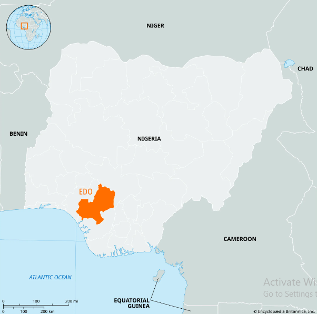
\includegraphics[width=0.9\linewidth]{Location of Edo in the Map.png}
    \caption{Location of Edo in the Map}
    \label{fig:loc of edo in map}
\end{figure}
\clearpage

Cultural landscapes played a pivotal role in shaping indigenous naming practices, as communities established connections between place names and cultural activities, rituals, and traditions. Sacred sites, ancestral shrines, and ritual grounds were often associated with specific place names, symbolizing their cultural and spiritual significance within the community.
The pre-colonial era witnessed the emergence of thriving urban centers, notably the ancient city of Benin, which served as the political, economic, and cultural capital of the Benin Kingdom. Place names within the city reflected its status as a center of power and innovation, with names honoring royal lineage, historical events, and royal titles\cite{egharevba1968short}.

% Assuming you have another figure to include; remember to replace 'imauuge.png' with the actual file name and provide a meaningful caption and label.
\begin{figure}[h!]
    \centering
    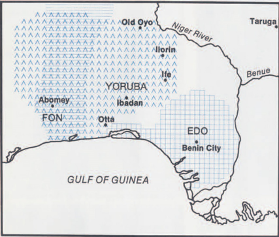
\includegraphics[width=0.9\linewidth]{imauuge.png}
    \caption{Illustrative Representation of a Cultural Landmark in Benin City}
    \label{fig:cultural_landmark_benin}
\end{figure}

The pre-colonial era in Edo and Benin City was characterized by indigenous naming practices deeply rooted in the linguistic diversity, cultural landscapes, and historical traditions of the region. Place names served as essential elements of cultural heritage, shaping the identity and historical evolution of the Benin Kingdom.
\subsubsection{Colonial era: Imposition of colonial names and cultural assimilation}
The colonial era marked a significant transition in the history of Edo and Benin City, characterized by the imposition of colonial names and the process of cultural assimilation under British colonial rule. This period saw profound changes in place naming practices as indigenous names were often replaced or anglicized to reflect colonial ideologies and administrative priorities.

Colonial administrators, missionaries, and explorers played key roles in renaming geographical features, urban centers, and administrative districts to align with British colonial interests and values. Indigenous place names were often deemed unpronounceable or culturally inappropriate by colonial authorities, leading to their replacement with English or European names\cite{Charles2007}.

During the colonial era, numerous geographical features, urban centers, and administrative districts in Edo and Benin City were renamed to align with British colonial interests and values. Some examples include:
Benin City: The capital city of the Benin Kingdom, originally known as Edo, was renamed Benin City during the colonial period to reflect British influence and establish administrative control over the region.
Geographical Features: Several geographical features, such as rivers, hills, and forests, were renamed to anglicized or European names. For example, the Ovia River might have been renamed to an English or European name by colonial authorities.
Urban Centers: Other urban centers within the region might have undergone renaming to reflect colonial influences. For instance, smaller towns or villages might have been given English or European names by colonial administrators.

Administrative Districts: Administrative districts and local government areas were often renamed to facilitate colonial governance and administrative control. Indigenous names for districts and regions might have been replaced with English or European names chosen by colonial authorities.
The imposition of colonial names was not merely a linguistic change but also a reflection of broader colonial policies aimed at asserting British authority and erasing indigenous identities. Place names became instruments of cultural domination and control, reinforcing colonial narratives of superiority and civilization over indigenous cultures\cite{Charles2007}.

The process of cultural assimilation during the colonial era further contributed to the transformation of place names in Edo and Benin City. Indigenous cultural practices, including language, religion, and governance systems, were systematically undermined and replaced with European norms and values. Place names served as symbolic markers of this cultural assimilation, reflecting the erasure of indigenous identities and the imposition of colonial hegemony.

Despite the imposition of colonial names, indigenous place names persisted in local memory and oral traditions, serving as resilient symbols of resistance and cultural resilience. Communities continued to use indigenous names in everyday speech and cultural practices, preserving their linguistic and cultural heritage in the face of colonial domination\cite{Charles2007}.
In summary, the colonial era in Edo and Benin City was characterized by the imposition of colonial names and the process of cultural assimilation under British colonial rule. Place names became contested sites of power and identity, reflecting the complex interplay between colonial domination and indigenous resistance.
\subsubsection{Post-colonial era: Reassertion of indigenous identities and urbanization trends}
The post-colonial era in Edo and Benin City witnessed a reassertion of indigenous identities and urbanization trends, leading to shifts in place naming practices and the resurgence of indigenous place names. This period marked a departure from colonial impositions, as communities sought to reclaim their cultural heritage and assert their identities in the newly independent nation of Nigeria\cite{reynolds}.

One of the significant trends during the post-colonial era was the resurgence of indigenous place names as symbols of cultural pride and identity. Communities across Edo and Benin City began to reclaim and revitalize indigenous names for geographical features, urban centers, and landmarks, reflecting a renewed appreciation for local history and traditions \cite{Davis1999african}.
Urbanization trends also influenced place naming practices during the post-colonial era, as rapid urban growth and development led to the emergence of new neighborhoods, streets, and landmarks. While some areas retained their colonial-era names, others were given indigenous names or names reflecting local historical figures, cultural symbols, or landmarks.

The post-colonial era also witnessed efforts to preserve and promote indigenous languages and cultural heritage in Edo and Benin City. Place names served as important linguistic and cultural markers, contributing to the revitalization of indigenous languages and the promotion of cultural diversity in urban spaces\cite{Davis1999african}.
Despite these efforts, challenges persist in the post-colonial era, including urbanization pressures, globalization influences, and socio-economic disparities that impact place naming practices and cultural identities in Edo and Benin City. Balancing modernization with cultural preservation remains a complex task for urban planners, policymakers, and communities seeking to navigate the dynamics of post-colonial urbanization.
The post-colonial era in Edo and Benin City marked a period of reassertion of indigenous identities, urbanization trends, and cultural revitalization. Place naming practices reflected these broader socio-cultural dynamics, serving as symbols of cultural pride, linguistic diversity, and historical continuity in the evolving urban landscapes of the region.

\section{Colonial influences: British administration and renaming initiatives}

The colonial period in Edo and Benin City ushered in a transformative era marked by the imposition of British administration and renaming initiatives, profoundly impacting the region's place naming practices and cultural landscapes. Under British colonial rule, colonial officials, missionaries, and explorers played pivotal roles in renaming geographical features, urban centers, and administrative districts to align with British colonial interests and values\cite{Afigbo1982}. 

These renaming initiatives were driven by various factors, including the perceived impracticality or cultural inappropriateness of indigenous place names in the eyes of colonial authorities. Indigenous names were often deemed unpronounceable or linguistically challenging, leading to their replacement with English or European names\cite{crowder2023british}. For instance, the capital city of the Benin Kingdom, originally known as Edo, was renamed Benin City during the colonial period to reflect British influence and assert colonial control over the region\cite{egharevba1968short}.

Moreover, geographical features such as rivers, hills, and forests underwent renaming to anglicized or European names chosen by colonial administrators. The Ovia River, for example, might have been renamed to an English or European name to erase indigenous associations and reinforce colonial hegemony. Similarly, urban centers and administrative districts were subjected to renaming initiatives aimed at erasing indigenous identities and imposing colonial control over the region's spatial organization \cite{Igbafe}.

These renaming efforts were not merely linguistic changes but reflected broader colonial policies of cultural domination and control. Place names became instruments of colonial authority, reinforcing narratives of British superiority and civilization over indigenous cultures. The renaming of geographical features and urban centers was part of a broader process of colonial territorialization, reshaping the region's cultural and geographical landscape to suit colonial interests\cite{Igbafe}.
The impact of colonial renaming initiatives extended beyond the surface level, influencing the region's socio-cultural dynamics and collective memory. Indigenous place names, deeply rooted in local languages, traditions, and histories, were marginalized or erased, leading to the loss of indigenous knowledge and cultural heritage. Moreover, the imposition of colonial names perpetuated narratives of colonial dominance and cultural erasure, contributing to the marginalization of indigenous communities and identities\cite{Igbafe}.

The colonial influences, particularly those of British administration and renaming initiatives, were pivotal factors shaping place name changes in Edo and Benin City during the colonial era. The imposition of colonial names reflected broader colonial agendas of cultural domination and control, leaving a lasting impact on the region's historical evolution and cultural identity\cite{aigimoukhuede2018benin}.

\subsubsection{Urban development: Infrastructure projects and city planning}

Urban development, characterized by infrastructure projects and city planning initiatives, has been a significant factor influencing place name changes in Edo and Benin City. As urban centers expanded and modernized, new neighborhoods, streets, and landmarks emerged, leading to the adoption of new place names and the renaming of existing ones\cite{nwokeji2010deatlanticizing,aigimoukhuede2018benin}.
Infrastructure projects, such as road construction, railway networks, and public utilities, have often necessitated the naming of new streets, squares, and districts. These projects, driven by urbanization trends and population growth, have contributed to the proliferation of place names reflecting contemporary urban landscapes and socio-economic realities.

City planning initiatives, undertaken by government authorities and urban planners, have also played a role in shaping place naming practices in Edo and Benin City. Master plans, zoning regulations, and urban renewal projects have influenced the naming of neighborhoods, parks, and public spaces, reflecting the vision and priorities of city officials\cite{bigon2009history}.
Furthermore, urban development projects have often been accompanied by efforts to commemorate historical figures, events, and cultural symbols through the naming of streets, monuments, and landmarks. These naming initiatives serve as markers of collective memory and identity, honoring the contributions of individuals and communities to the city's history and development\cite{nwokeji2010deatlanticizing}.
However, urban development projects have also been contentious, leading to debates over the preservation of historical and cultural heritage. In some cases, the demolition of historic neighborhoods or landmarks has sparked protests and calls for the preservation of indigenous place names and cultural landscapes\cite{nwokeji2010deatlanticizing}.
The urban development, characterized by infrastructure projects and city planning initiatives, has been a significant factor influencing place name changes in Edo and Benin City. While these initiatives reflect the dynamic nature of urban growth and development, they also raise questions about the preservation of historical and cultural heritage in the face of rapid urbanization\cite{aigimoukhuede2018benin}.
\subsubsection{Cultural dynamics: Language shifts, migration patterns, and socio-political changes}
Cultural dynamics, encompassing language shifts, migration patterns, and socio-political changes, have significantly influenced place name changes\cite{lanati2021cultural}. These factors reflect the evolving socio-cultural landscape of the region and its impact on the naming practices of communities\cite{aigimoukhuede2018benin}.
Language shifts, driven by historical processes of colonization, urbanization, and globalization, have influenced place naming practices in Edo and Benin City. As linguistic landscapes evolve, indigenous languages may experience shifts in usage, leading to changes in the naming of geographical features, urban centers, and landmarks\cite{egharevba1968short}.

Migration patterns have also shaped place naming practices, as communities move and settle in new areas, bringing with them their linguistic and cultural traditions. Immigrant communities may establish new neighborhoods, streets, and cultural institutions, reflecting their cultural heritage and identity in the naming of these spaces.

Moreover, socio-political changes, including shifts in governance, power dynamics, and political ideologies, have influenced place name changes in Edo and Benin City. Historical events, such as independence movements, regime changes, and civil unrest, may lead to the renaming of streets, squares, and public buildings to reflect new political realities and aspirations\cite{aigimoukhuede2018benin,egharevba1968short}.

Cultural dynamics also intersect with issues of identity and representation, as marginalized communities seek to assert their cultural heritage and reclaim their place in the city's narrative. Indigenous groups may advocate for the preservation of indigenous place names and the recognition of their contributions to the city's history and development\cite{egharevba1968short}.
However, cultural dynamics can also be contested, reflecting tensions between different linguistic, ethnic, and socio-economic groups. Place naming practices may become sites of negotiation and conflict, as communities vie for recognition and representation in the city's public spaces.

The cultural dynamics, including language shifts, migration patterns, and socio-political changes, have been significant factors influencing place name changes in Edo and Benin City. These dynamics reflect the complex interplay of historical, social, and cultural forces shaping the region's naming practices and identity.
